\documentclass{article}


% if you need to pass options to natbib, use, e.g.:
%     \PassOptionsToPackage{numbers, compress}{natbib}
% before loading neurips_2023

% ready for submission
\usepackage[final]{neurips_2023}

% to avoid loading the natbib package, add option nonatbib:
%    \usepackage[nonatbib]{neurips_2023}


\usepackage[utf8]{inputenc} % allow utf-8 input
\usepackage[T1]{fontenc}    % use 8-bit T1 fonts
\usepackage{hyperref}       % hyperlinks
\usepackage{url}            % simple URL typesetting
\usepackage{booktabs}       % professional-quality tables
\usepackage{amsfonts}       % blackboard math symbols
\usepackage{nicefrac}       % compact symbols for 1/2, etc.
\usepackage{microtype}      % microtypography
\usepackage{xcolor}
\usepackage{amsmath}
\usepackage{graphicx}         % colors


\title{MLPC Report Task 2 - Data Exploration}


% The \author macro works with any number of authors. There are two commands
% used to separate the names and addresses of multiple authors: \And and \AND.
%
% Using \And between authors leaves it to LaTeX to determine where to break the
% lines. Using \AND forces a line break at that point. So, if LaTeX puts 3 of 4
% authors names on the first line, and the last on the second line, try using
% \AND instead of \And before the third author name.


\author{% 
  Team Park \AND
  Author Oliver König
  \And
  Author Daniel Hörtenhuber
  \And 
  Author Wolfram Laube
}


\begin{document}


\maketitle


\begin{contributions}
  Section 1, infrastructure, layout: Wolfram Laube - Section 2, 3: Daniel Hörtenhuber - Section 4: Oliver König
\end{contributions}


\section{Data Consistency \& Quality}

\subsection{Feature Statistics Examination}

Our initial step in assessing the data's consistency and quality involved a detailed examination of the feature statistics across the entire dataset. This approach allows us to identify potential outliers, inconsistencies, and wrongly labeled audio snippets without the need to listen to each recording individually. Here's how we conducted this examination:

\subsubsection{Methodology:}

\begin{enumerate}
    \item \textbf{Descriptive Statistics}: We calculated basic descriptive statistics for each feature, including mean, median, standard deviation, and interquartile range (IQR). These metrics provide insights into the central tendency and spread of the data, helping identify features with abnormal distributions.
    \item \textbf{Outlier Detection}: By applying the IQR method, we identified outliers as those points lying below \(Q1 - 1.5 \times \text{IQR}\) or above \(Q3 + 1.5 \times \text{IQR}\), where \(Q1\) and \(Q3\) are the first and third quartiles, respectively. This method helped pinpoint samples with feature values significantly deviating from the bulk of the data.
    \item \textbf{Visualization}: We utilized box plots and histograms for each feature to visually inspect their distributions. Box plots were particularly useful in spotting outliers, while histograms allowed us to observe the shape of the distributions, revealing any skewness or multimodality.
\end{enumerate}

\subsubsection{Findings:}

\begin{itemize}
    \item \textbf{Outliers and Anomalies}: Several features, particularly those related to spectral properties such as spectral centroid and rolloff, exhibited outliers. These outliers could indicate recordings that are either mislabeled or possess unique characteristics (e.g., background noise, recording errors) diverging from typical samples.
    \item \textbf{Abnormal Distributions}: Some features showed highly skewed distributions, suggesting the presence of recordings that might not be representative of the dataset's overall characteristics. For instance, features measuring energy and loudness had distributions skewed towards lower values, potentially indicating recordings with very low volume or silence.
    \item \textbf{Potential Mislabelings}: In examining the relationship between features and labels, we noted instances where the feature statistics for certain labels did not align with expectations. This discrepancy could suggest mislabelings, such as a word being incorrectly categorized or background noise being labeled as a speech command.
\end{itemize}

\subsubsection{Implications and Next Steps:}

\begin{itemize}
    \item \textbf{Data Cleaning}: The identified outliers and potential mislabelings necessitate a review and potential cleaning of the dataset to ensure the accuracy of our model. This step may involve reevaluating the labeling process or excluding certain anomalies from the training set.
    \item \textbf{Feature Engineering}: Given the abnormal distributions observed in some features, we may consider feature transformation (e.g., logarithmic transformation) or normalization techniques (e.g., scaling) to mitigate their effects and improve model performance.
    \item \textbf{Further Analysis}: To strengthen our understanding of the data's quality, additional analyses, such as examining feature variance and conducting cluster analysis, could provide further insights into the dataset's structure and any underlying issues.
\end{itemize}

\subsection{Listening and Bias Identification}

Listening to a subset of the recordings has provided valuable insights into the dataset, particularly in terms of accent and gender distribution. These biases could influence model performance and its ability to generalize across different user groups.

\subsubsection{Findings:}

\begin{itemize}
    \item \textbf{Accent Bias}: Analysis of a random sample of approximately 30\% of the data
    revealed a significant bias towards foreign accents, with a ratio of 31 foreign to
    19 domestic (German) accents.
    This imbalance may impact the model’s ability to accurately recognize commands spoken
    with a German accent.
    \item \textbf{Gender Bias}: Anotheer random sample of same size showed a gender distribution of 33 males to 17 females. This skew towards male voices could lead to lower accuracy or performance when recognizing commands from female speakers.
\end{itemize}

\begin{figure}[!ht]
	\centering
	\includegraphics[scale=0.5]{fig/biases}
	\vspace{-0.3cm}
	\caption{Biases.}
	\label{fig:Biases}
	\vspace{-0.1cm}
\end{figure}


\subsubsection{Recommendations:}

\begin{itemize}
    \item \textbf{Data Collection}: To mitigate these biases, additional data collection efforts should focus on increasing the number of recordings from female speakers and those with a German accent. This will help in balancing the dataset and improving the model's robustness.
    \item \textbf{Model Training}: Consider using techniques such as stratified sampling during training to ensure that the model learns equally well from all categories of data, regardless of accent or gender.
\end{itemize}

\subsection{``Other'' Sounds Analysis}

Listening to some of the sounds labeled as “Other” provided insights into the types of non-speech audio included in the dataset. This category is crucial for ensuring the model can appropriately handle irrelevant sounds when deployed in real-world environments.

\subsubsection{Findings:}

\begin{itemize}
    \item \textbf{Types of Sounds}: The "Other" category includes a variety of sounds typically found in household settings, such as background noise, household appliances, and television audio. These sounds are representative of everyday noises likely to be encountered.
\end{itemize}

\begin{figure}[!ht]
	\centering
	\includegraphics[scale=0.25]{fig/other}
	\vspace{-0.3cm}
	\caption{'Other' Sounds.}
	\label{fig:Other}
	\vspace{-0.1cm}
\end{figure}

\subsubsection{Implications:}

\begin{itemize}
    \item \textbf{Model Training}: Training the model to distinguish these "Other" sounds from speech commands is essential for preventing false activations and improving user experience. The diversity of sounds within this category suggests the need for robust feature extraction techniques that can capture a wide range of audio characteristics.
\end{itemize}

\section{Label Characteristics}

\subsection{Grouping Strategy}

Given the dataset's nature involving speech commands, effective grouping of the labels is crucial for both practical application and computational efficiency. Here’s a suggested approach for grouping:

\subsubsection{Methodology:}

\begin{itemize}
    \item \textbf{Semantic Similarity}: Group words based on their semantic meaning and usage in common speech scenarios. For example, commands like "an" and "aus" could be grouped under a category like "Commands."
\end{itemize}

\subsubsection{Proposed Groups:}

\begin{itemize}
    \item \textbf{Devices}: Includes "Fernseher", "Radio", "Licht" and "Alarm".
    \item \textbf{Appliances}: Includes "Heizung", "Lüftung", "Ofen" and "Staubsauger".
    \item \textbf{Commands}: Includes "an" and "aus".
    \item \textbf{Status}: Includes "warm", "offen".
    \item \textbf{Objects}: Includes "Leitung", "Spiegel", "Brötchen", "Haus" and "Schraube".
    \item \textbf{Miscellaneous}: All remaining words that do not neatly fit into the above categories but are still relevant for broad command recognition. Here includes "kann", "nicht", "wunderbar" and "other".
\end{itemize}

\subsection{Class Balance Assessment}

Class balance is critical in training machine learning models to prevent biases toward more frequent classes.

\subsubsection{Methodology:}

\begin{enumerate}
    \item \textbf{Quantitative Analysis}: Calculate the variance of each class in the dataset. Use bar charts to visually represent these distributions to quickly identify any imbalance.
    \item \textbf{Assess Impact}: Discuss how the imbalance might affect model training, particularly if some classes are underrepresented, potentially leading to poorer model performance on these classes.
\end{enumerate}

\subsubsection{Findings:}

\begin{itemize}
    \item \textbf{Imbalance Details}: The bar chart used to visualize these groups shows a noticeable imbalance between them. Especially Status and Commands are underrepresented. An obvious indicator of this imbalance is the Coefficient of Variance, which comes out to be 38\%.
    \item \textbf{Strategies for Mitigation}: Data augmentation or collecting more data, especially for the minority classes are potential approaches to balance the classes to improve model performance.
\end{itemize}

\begin{figure}[!ht]
	\centering
	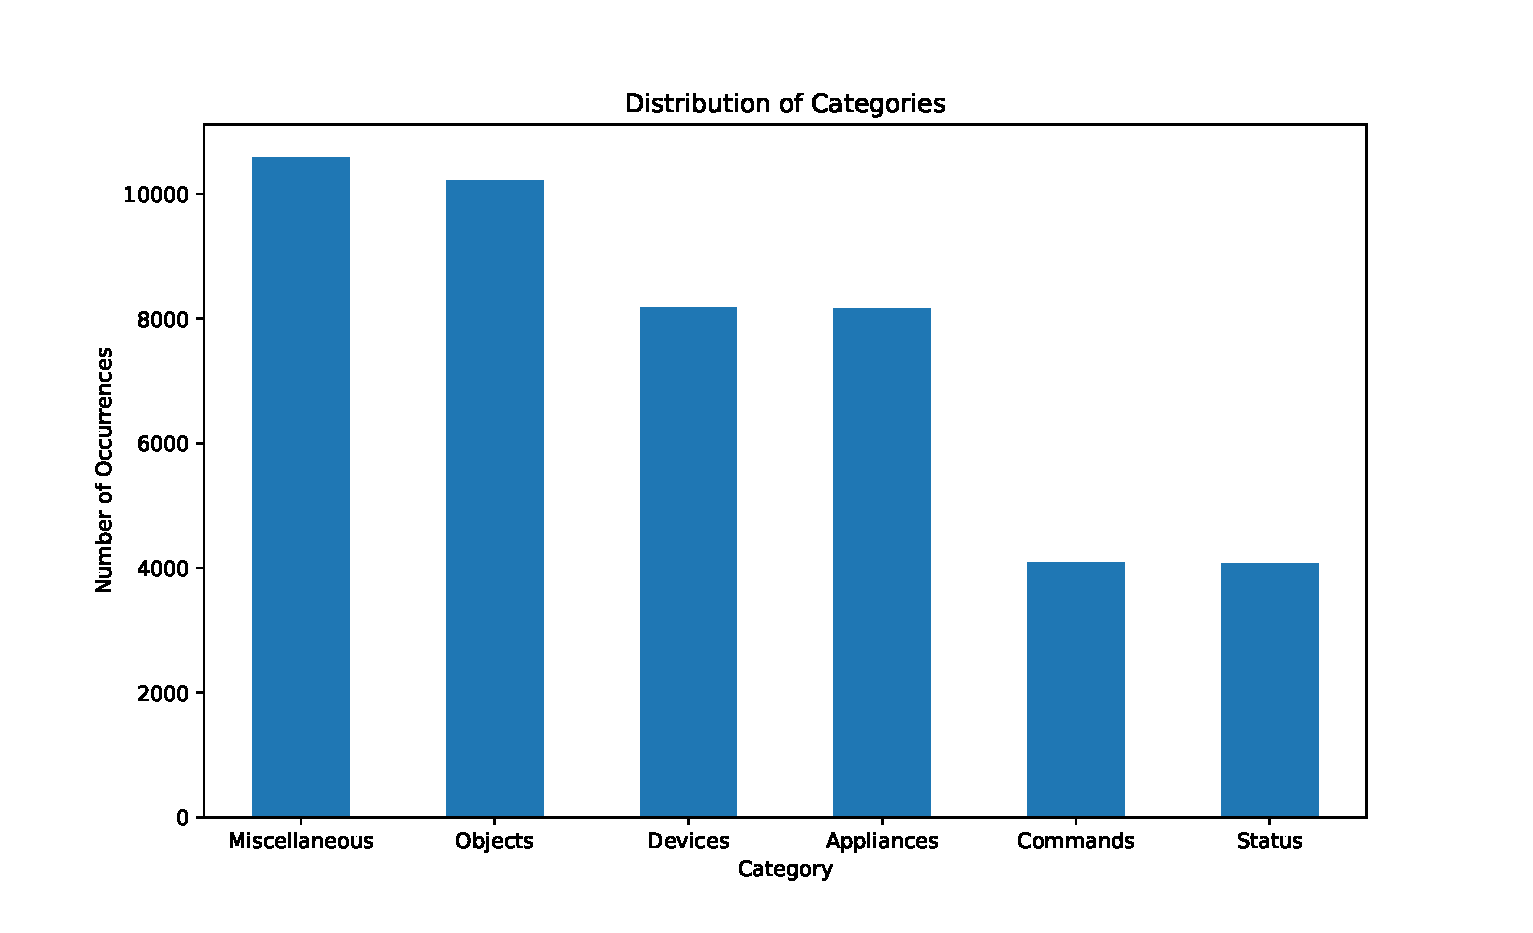
\includegraphics[scale=0.3]{fig/categories_dist}
	\vspace{-0.3cm}
	\caption{Categories Distribution.}
	\label{fig:CategoriesDistribution}
	\vspace{-0.1cm}
\end{figure}
\section{Feature Characteristics}

\subsection{Feature Distribution Analysis}

Understanding the distribution of features within our dataset is critical for identifying potential preprocessing steps and informing model selection.

\subsubsection{Methodology:}

We utilized histograms to examine the distributions of pre-computed audio features across the dataset. This visualization aids in identifying features with non-normal distributions, which could potentially skew the performance of many machine learning algorithms that assume normally distributed data.

\subsubsection{Findings:}

\begin{itemize}
    \item \textbf{Skewed Distributions}: Certain features, especially those related to frequency and energy, exhibited skewed distributions. This skewness indicates that some preprocessing, such as log transformation or normalization, might be necessary to align these features more closely with a normal distribution.
    \item \textbf{Normal Distributions}: Mel-scaled energies, MFCCs, Centroid, Bandwidth, and Contrasts follow a normal distribution. These features capture aspects like frequency perception, sound "center of mass", frequency spread, and the difference between peak and valley energies in spectral bands, reflecting the tonal and noise characteristics of the sound.
\end{itemize}

\begin{figure}[!ht]
	\centering
	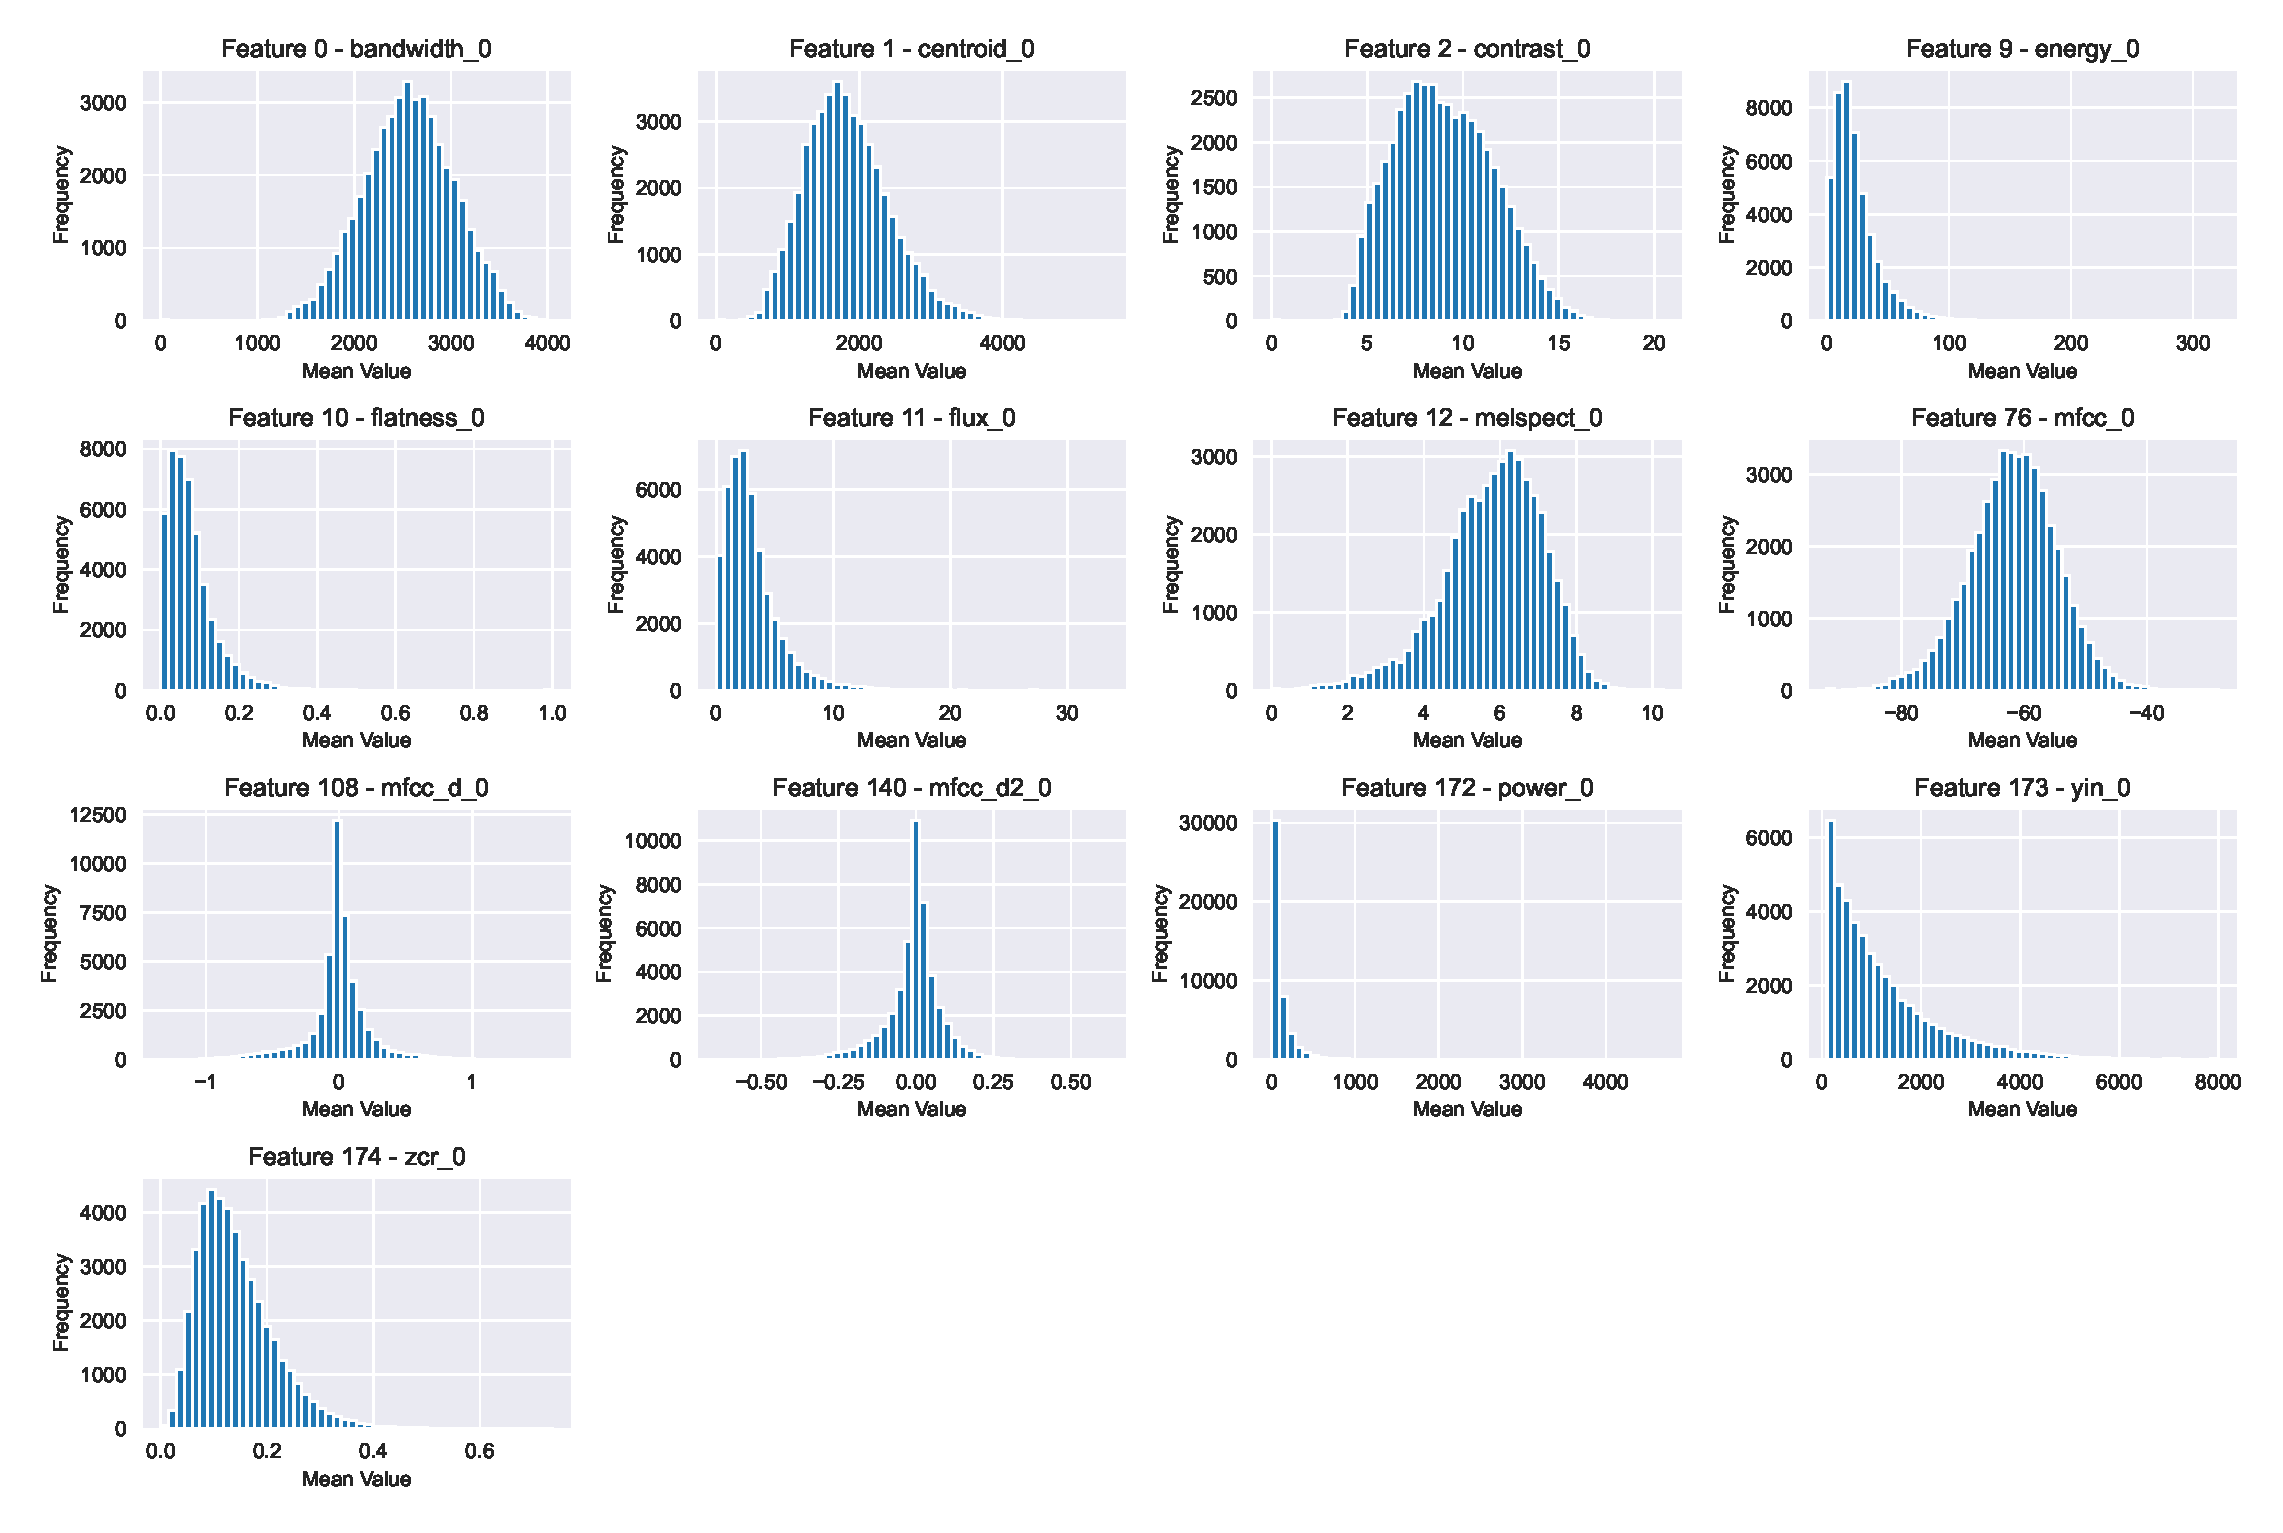
\includegraphics[scale=0.3]{fig/feature_dist}
	\vspace{-0.3cm}
	\caption{Feature Distribution.}
	\label{fig:FeatureDistribution}
	\vspace{-0.1cm}
\end{figure}


\subsection{Correlation and Redundancy}

Analyzing the correlation between features is essential to identify redundant information that could be pruned to simplify the model and reduce the risk of overfitting.

\subsubsection{Methodology:}

We applied Pearson's correlation coefficient to assess linear relationships between pairs of features. A heatmap visualization helped us quickly identify areas of high correlation, indicative of redundant information.

\subsubsection{Findings:}

\begin{itemize}
    \item \textbf{Highly Correlated Features}: Several pairs of features related to spectral properties showed high correlation (coefficients above 0.9), suggesting redundancy. For instance, mel-scaled energies, power, energy and spectral flux were often closely aligned across samples.
    \item \textbf{Redundancy Reduction}: Based on these findings, we recommend a dimensionality reduction technique, such as Principal Component Analysis (PCA), to eliminate redundant features while preserving the variance within the dataset.
\end{itemize}

\begin{figure}[!ht]
	\centering
	\begin{minipage}{0.49\textwidth}
		\centering
		\includegraphics[scale=0.3]{fig/heatmap_single}
		\caption{Correlation - All features of single frame.}
		\label{fig:HeatmapSingle}
	\end{minipage}\hfill
	\begin{minipage}{0.49\textwidth}
		\centering
		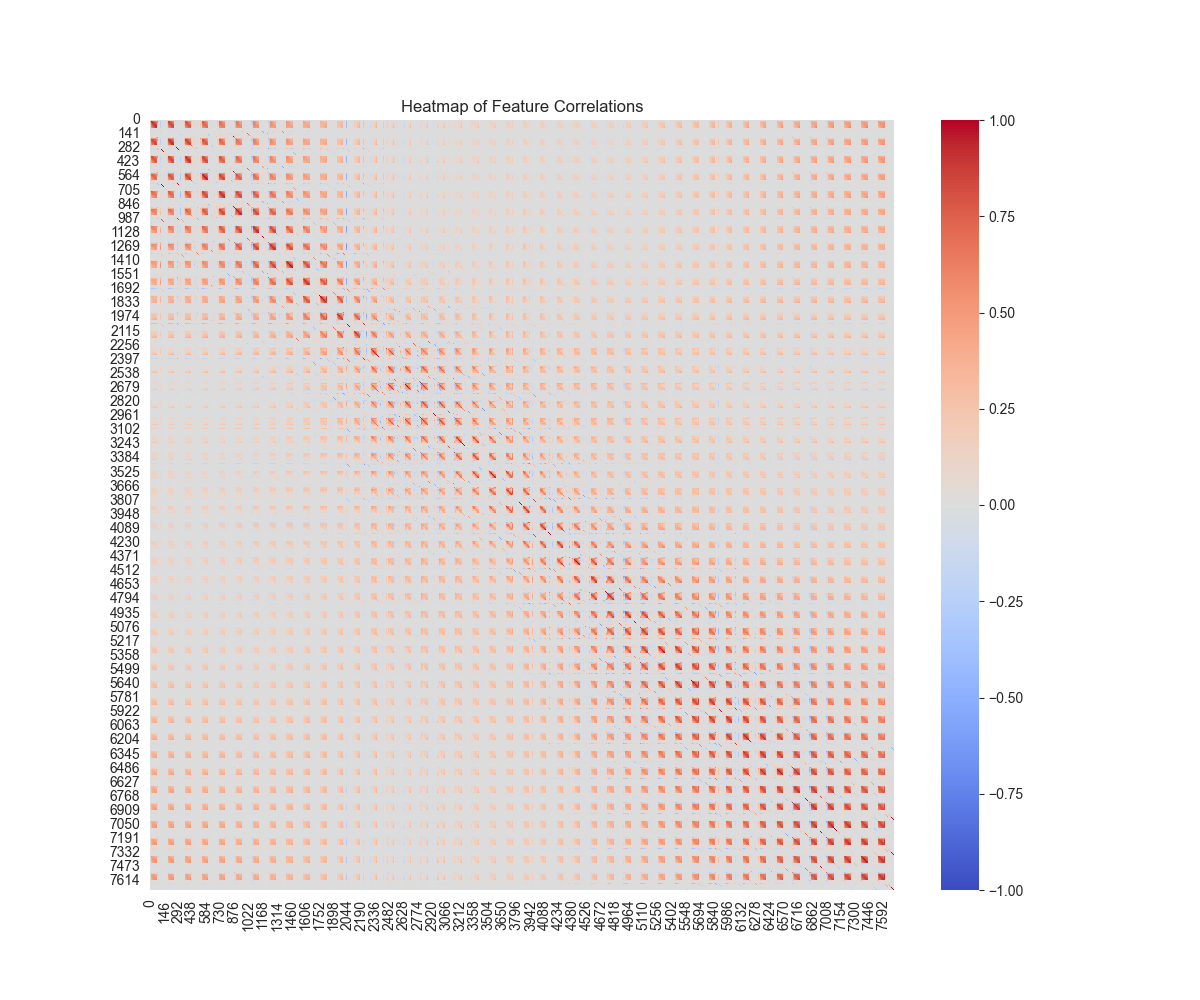
\includegraphics[scale=0.3]{fig/heatmap_all}
		\caption{Correlation - All feature across all frames.}
		\label{fig:HeatmapAll}
	\end{minipage}
\end{figure}

\subsection{Speaker Variation}

Investigating whether the distribution of features varies significantly across different speakers is crucial for ensuring our model's robustness to speaker variability.

\subsubsection{Methodology:}

For this analysis, we grouped the data by speaker identity and then analyzed the variance within feature distributions across these groups.
This approach helps us to understand if and how much the speaker's identity might influence the observed feature values.

\subsubsection{Findings:}

\begin{itemize}
    \item \textbf{Variation Across Speakers}: Preliminary analysis suggests variability in certain features, particularly those related to pitch and timbre, across different speakers.
    This variability underscores the importance of including speaker normalization techniques in our preprocessing pipeline to mitigate these effects.
    \item \textbf{Normalization Techniques}: Techniques such as cepstral mean normalization (CMN)\footnote{https://en.wikipedia.org/wiki/Cepstral\textunderscore mean\textunderscore and\textunderscore variance\textunderscore normalization} or c (VAD)\footnote{https://en.wikipedia.org/wiki/Voice\textunderscore activity\textunderscore detection} could be employed to reduce the impact of speaker variability on feature distributions.
\end{itemize}

%\begin{figure}[!ht]
%	\centering
%	\begin{minipage}{0.49\textwidth}
%		\centering
%		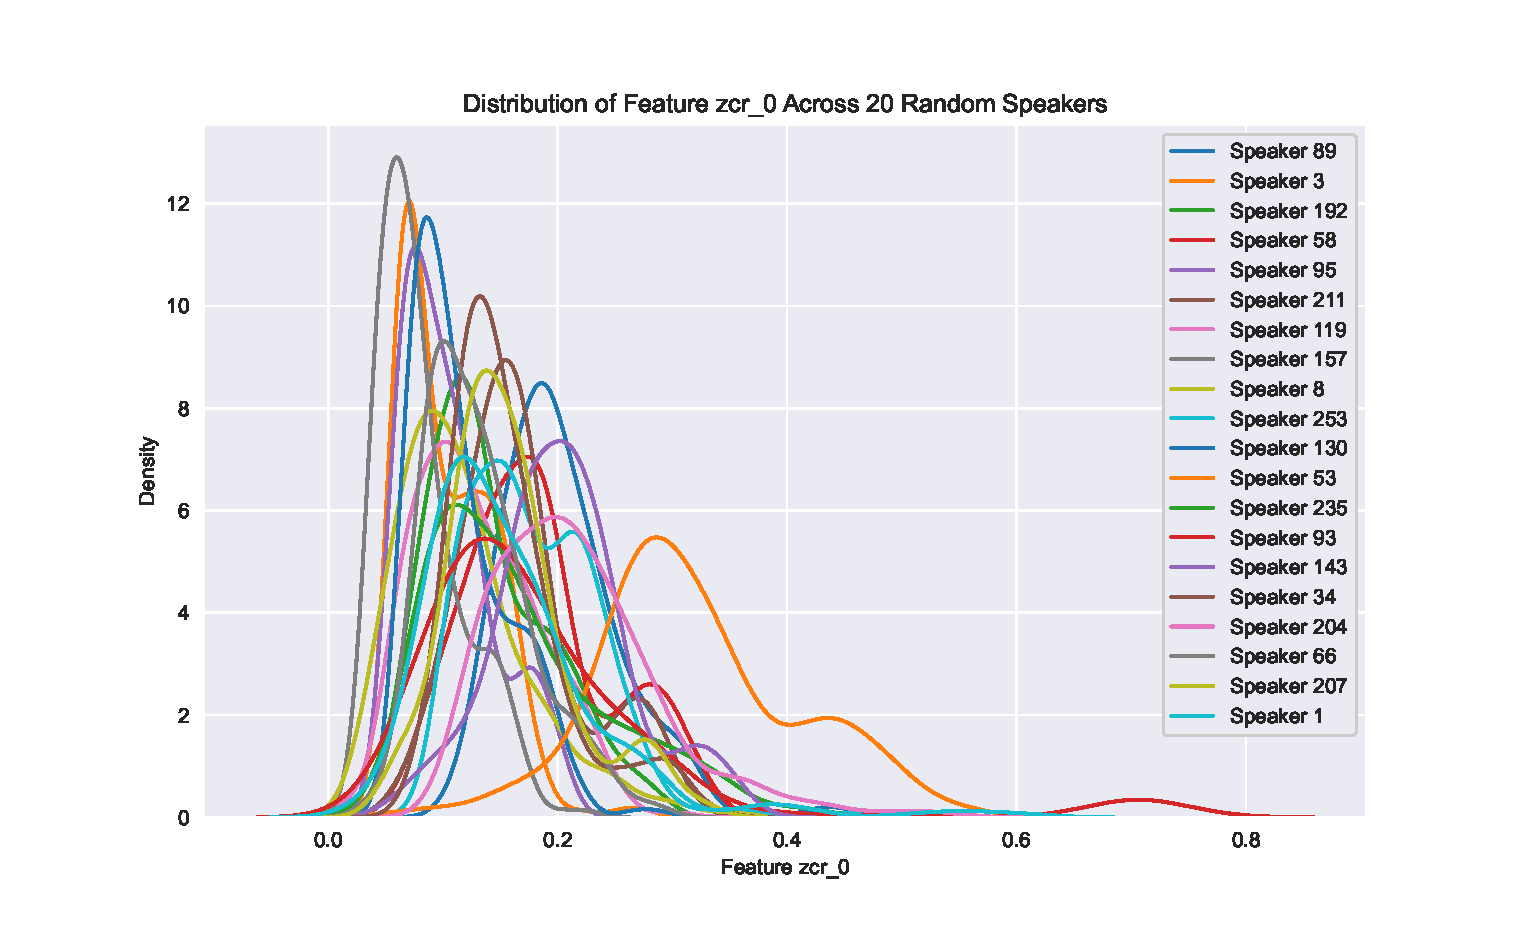
\includegraphics[scale=0.3]{fig/speakers_zcr0}
%		\caption{Speakers ZCR0}
%		\label{fig:SpeakersZcr0}
%	\end{minipage}\hfill
%	\begin{minipage}{0.49\textwidth}
%		\centering
%		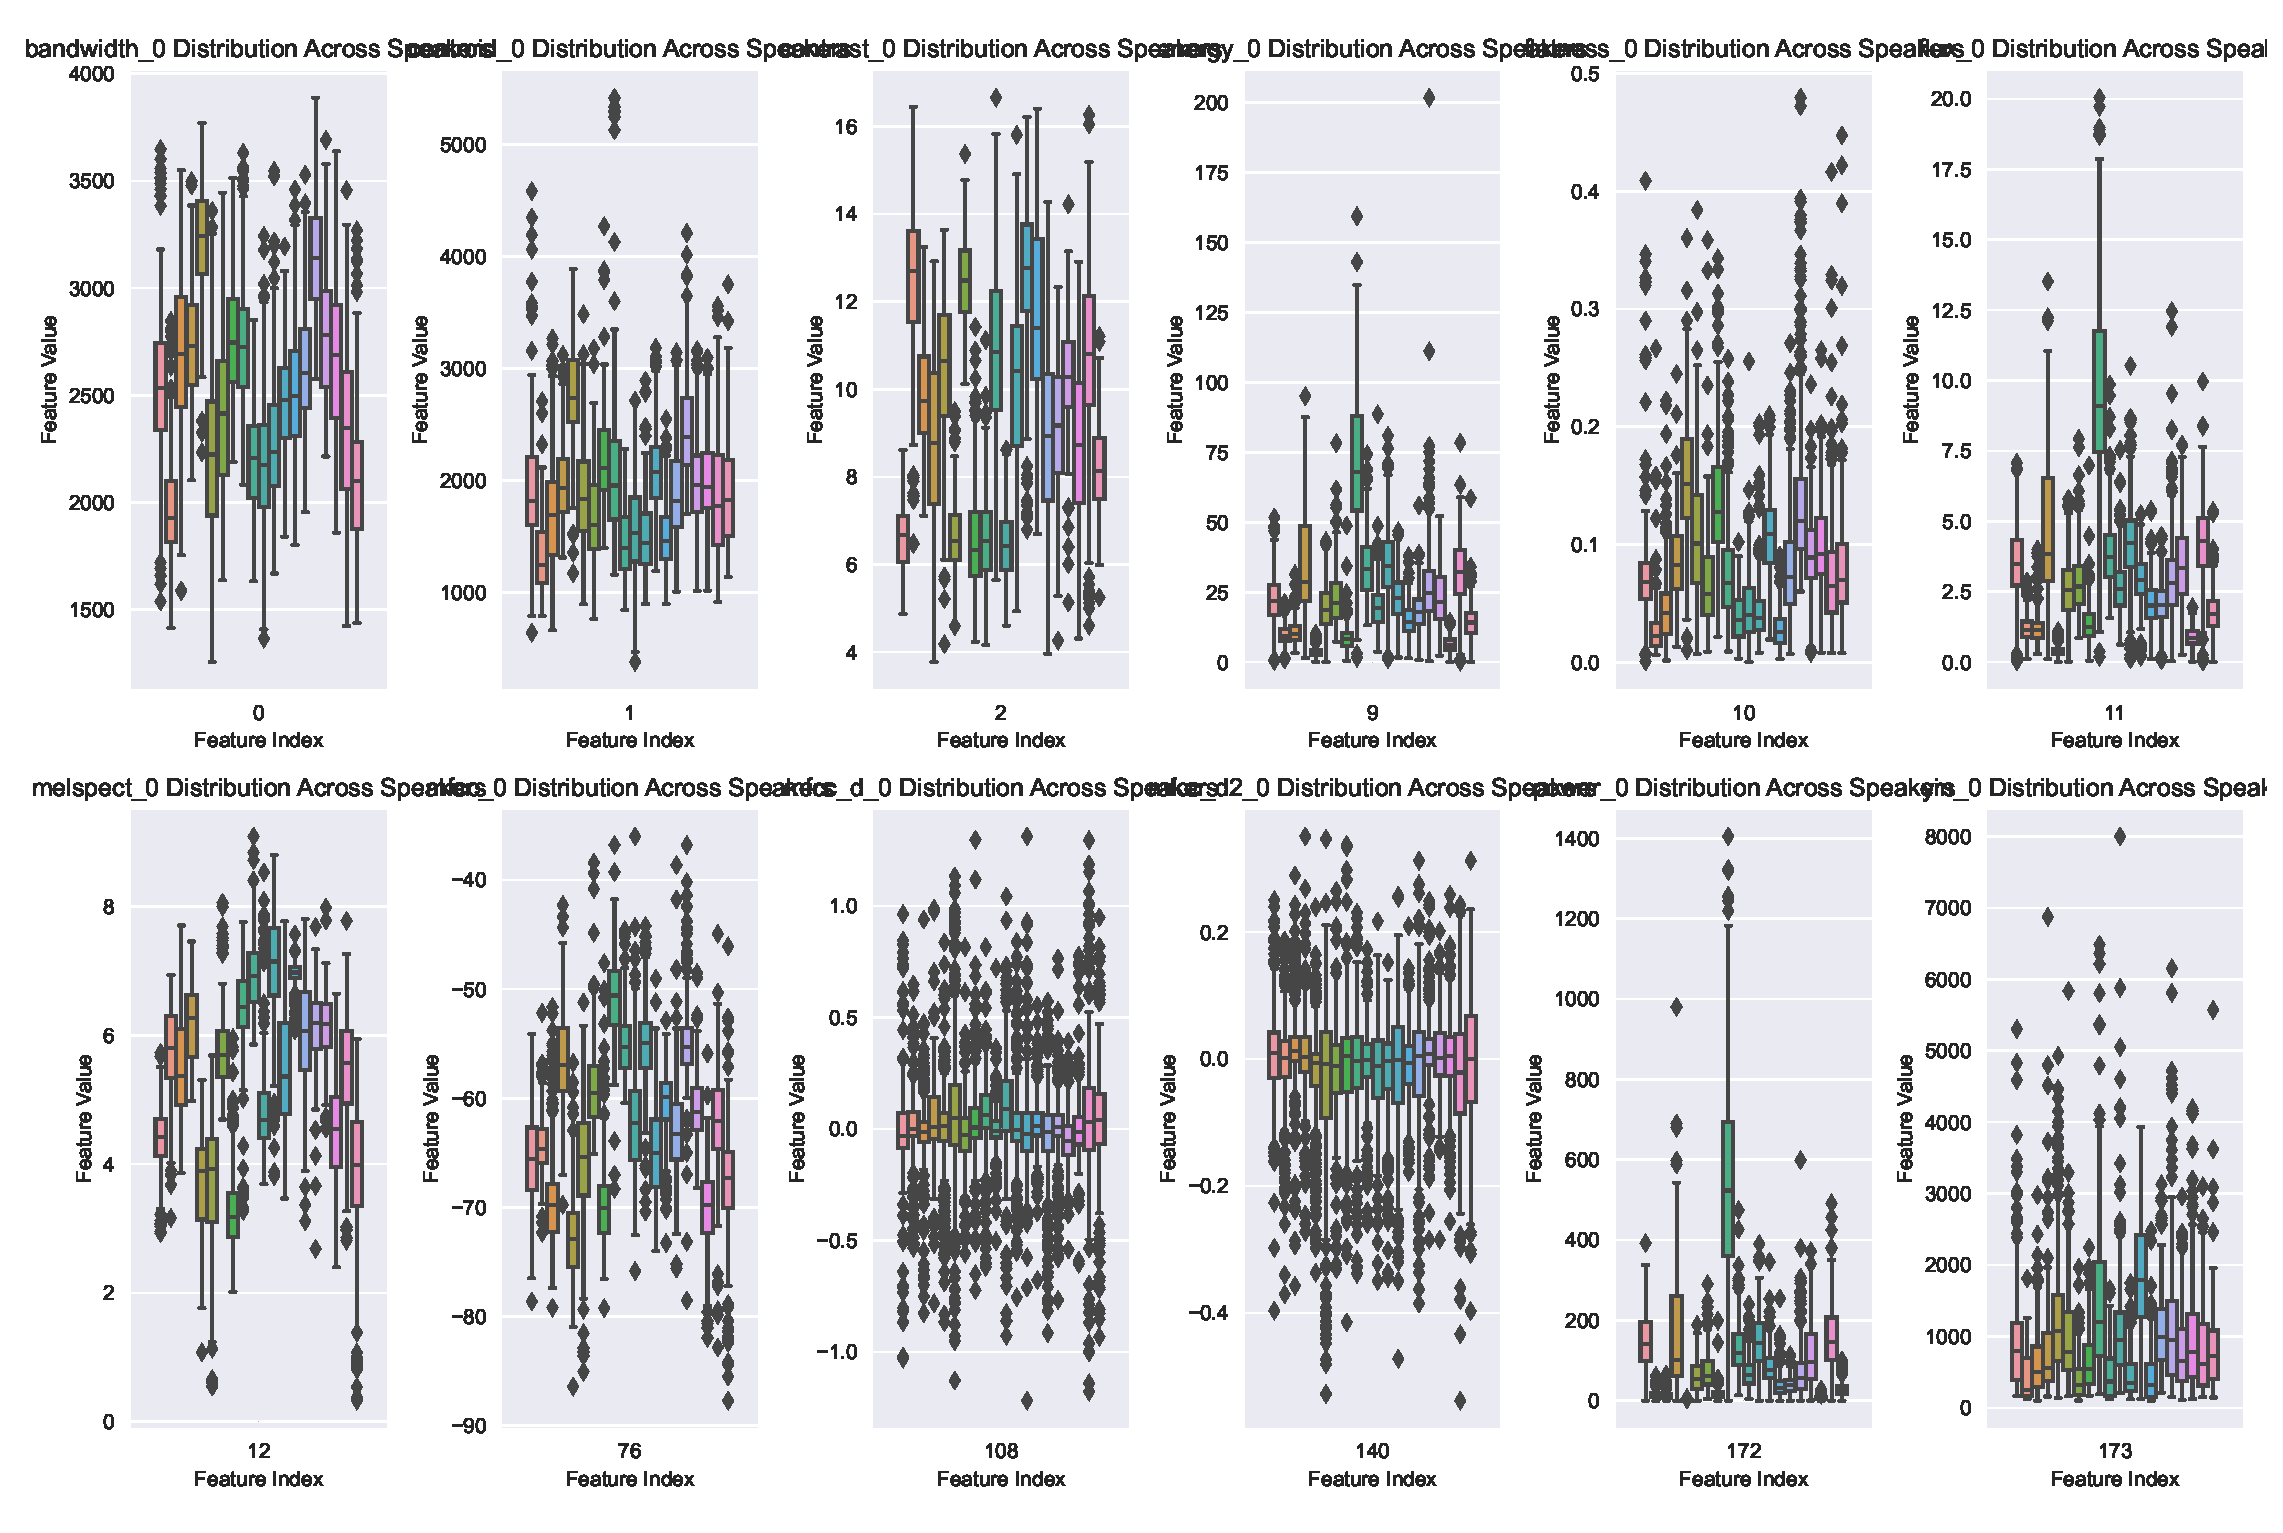
\includegraphics[scale=0.3]{fig/speakers_dist}
%		\caption{Additional Image Description.}
%		\label{fig:Speakers Dist}
%	\end{minipage}
%\end{figure}

\begin{figure}[!ht]
	\centering
	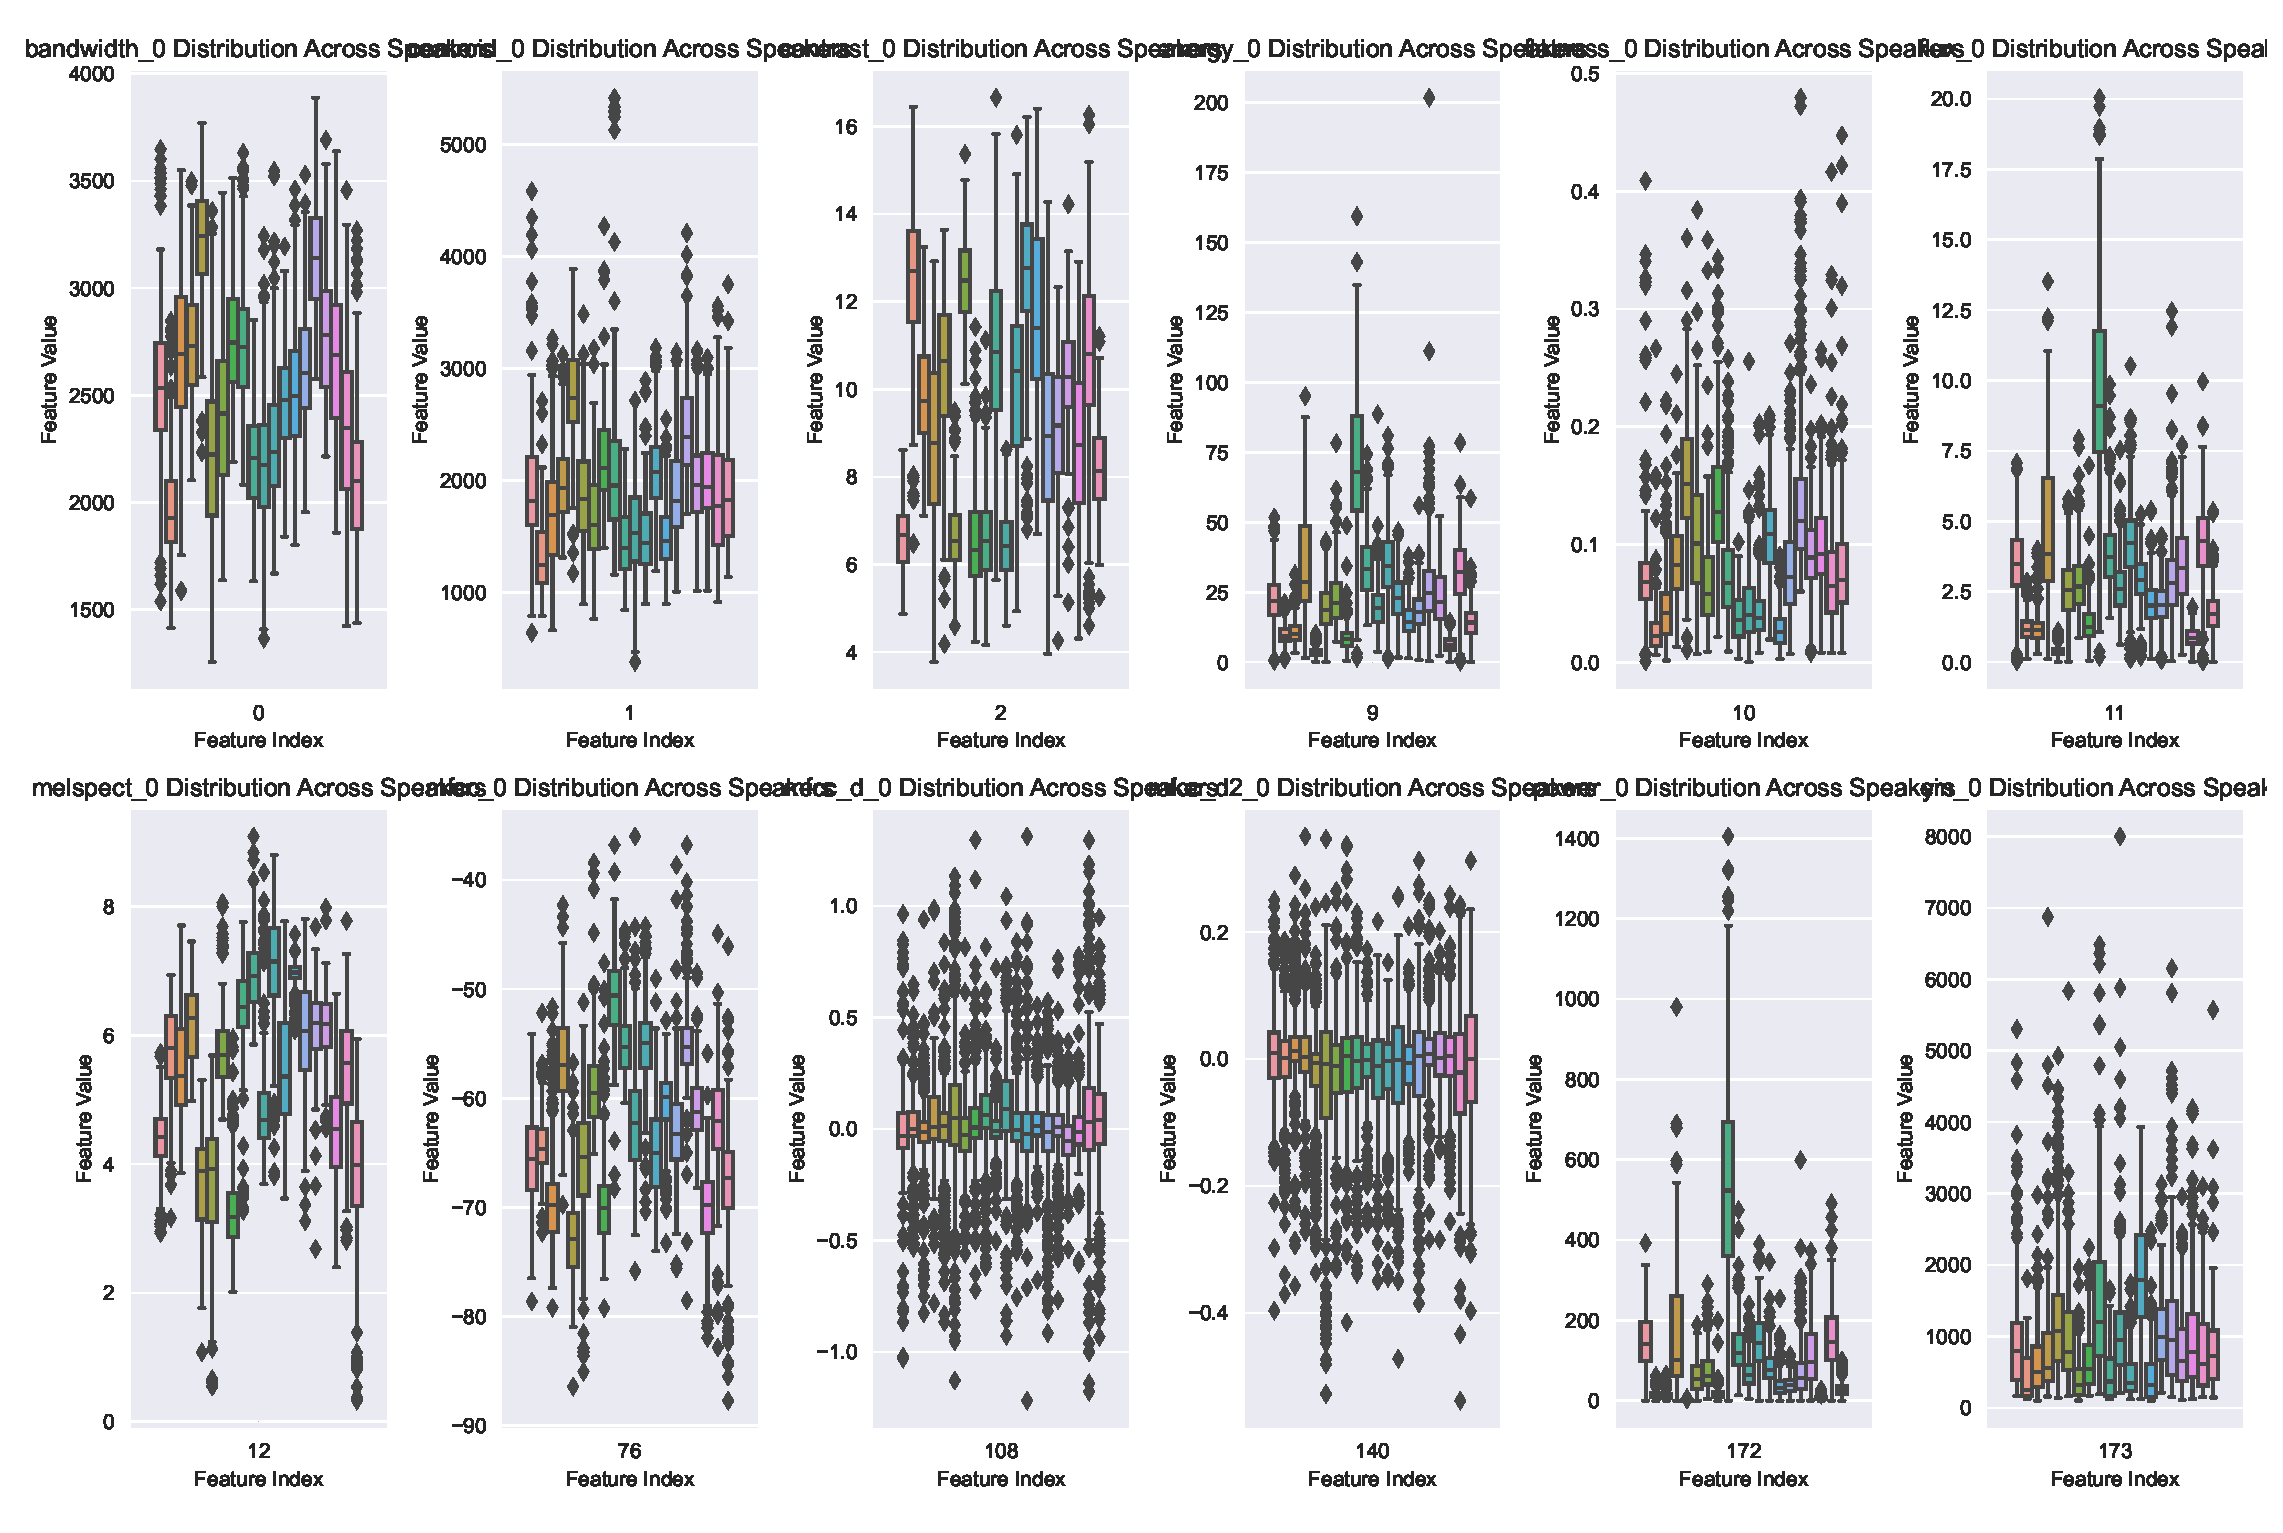
\includegraphics[scale=0.3]{fig/speakers_dist}
	\vspace{-0.3cm}
	\caption{Speakers Distribution.}
	\label{fig:SpeakersDistribution}
	\vspace{-0.1cm}
\end{figure}

\begin{figure}[!ht]
	\centering
	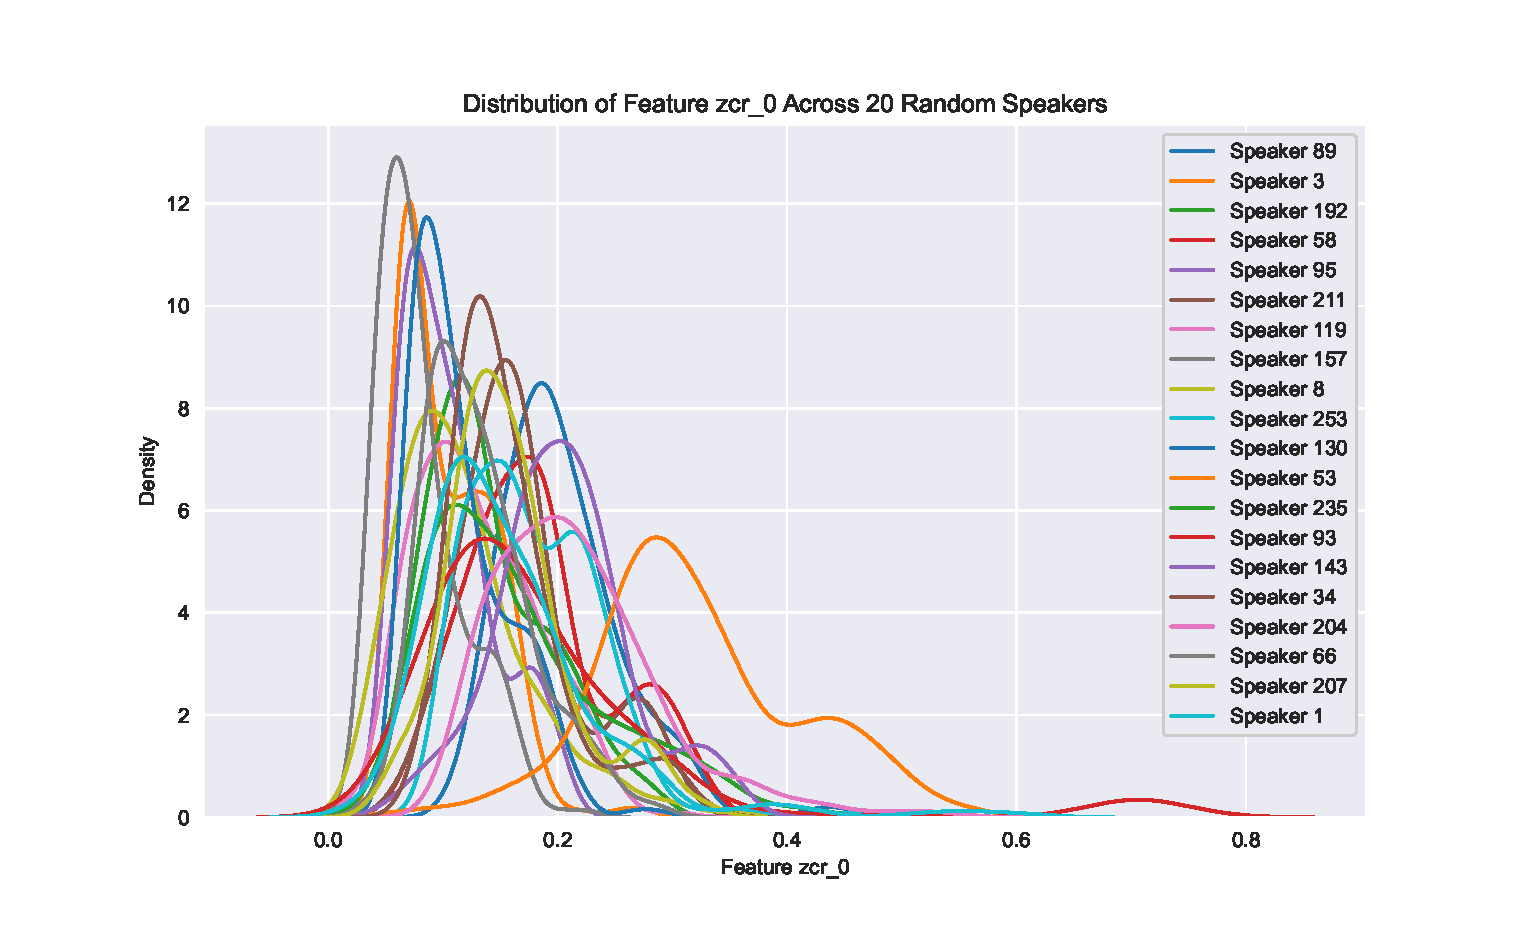
\includegraphics[scale=0.3]{fig/speakers_zcr0}
	\vspace{-0.3cm}
	\caption{Speakers ZCR0.}
	\label{fig:SpeakersZCR0}
	\vspace{-0.1cm}
\end{figure}
\section{Feature / Label Agreement}

\subsection{Useful Features for Classification}

Identifying features that are most predictive of labels is crucial for effective model training. This section discusses the correlation between features and labels to determine which features contribute most significantly to the classification task.

\subsubsection{Methodology:}

\begin{enumerate}
    \item \textbf{Feature Importance Analysis}: Utilize techniques such as feature importance scores from tree-based models (e.g., Random Forests) and mutual information to quantify the contribution of each feature to the prediction accuracy.
    \item \textbf{Correlation Analysis}: Compute correlation coefficients between features and labels to identify direct relationships that can inform feature selection and model refinement.
\end{enumerate}

\subsubsection{Findings:}

\begin{itemize}
    \item \textbf{Significant Features}: Features such as Mel-frequency cepstral coefficients (MFCCs), spectral contrast, and zero-crossing rate have been identified as highly predictive, showing strong correlations with specific speech commands.
    \item \textbf{Model Implications}: The identification of key features will guide the feature selection process, ensuring that the model focuses on the most informative attributes, thereby improving efficiency and prediction accuracy.
\end{itemize}

\begin{figure}[!ht]
	\centering
	\begin{minipage}{0.49\textwidth}
		\centering
		\includegraphics[scale=0.3]{fig/scatterplot_cluster_natural_tsne}
		\caption{Clustering - Natural Clusters inferred by K-Means.}
		\label{fig:ClusterNatural}
	\end{minipage}\hfill
	\begin{minipage}{0.49\textwidth}
		\centering
		\includegraphics[scale=0.3]{fig/scatterplot_cluster_categories_tsne}
		\caption{Clustering - Clusters inferred by categorization \textit{as is}.}
		\label{fig:ClusterCategorized}
	\end{minipage}
\end{figure}


\subsection{Similar Words Feature Distribution}

Analyzing how features distribute among phonetically similar words is essential for ensuring the model can distinguish between such words effectively.

\subsubsection{Methodology:}

\begin{enumerate}
    \item \textbf{Comparative Analysis}: Examine the feature distributions for pairs or sets of similar-sounding words to assess whether their feature spaces significantly overlap.
    \item \textbf{Statistical Testing}: Use statistical tests such as the Kolmogorov-Smirnov test to determine if the distributions of features for similar words are statistically different.
\end{enumerate}

\subsubsection{Findings:}

\begin{itemize}
    \item \textbf{Distribution Overlap}: Preliminary analysis has shown that certain similar-sounding words (e.g., "haus" vs. "aus") exhibit overlapping feature distributions, which could pose challenges in classification tasks.
    \item \textbf{Feature Engineering Needs}: These findings suggest a need for advanced feature engineering techniques or the incorporation of contextual information to improve the distinguishability of similar-sounding words.
\end{itemize}


\section{Conclusion}

This report has thoroughly investigated various aspects of the speech command dataset through comprehensive data analysis, exploring data consistency, label characteristics, feature properties, and the relationship between features and labels. Here are the key conclusions and recommendations:

\subsection{Summary of Key Findings}

\begin{itemize}
    \item \textbf{Data Quality}:
    The investigation revealed several minor data quality issues,
    including outliers and potential mislabelings. Enhanced data cleaning and verification
    are recommended to improve dataset integrity.
    \item \textbf{Label and Feature Analysis}:
    The analysis identified imbalances in class distribution and highlighted the need
    for thoughtful grouping of labels to enhance model performance.
    Significant correlations between certain features and labels were found,
    underscoring their importance for classification tasks.
    \item \textbf{Feature Redundancy and Speaker Variability}:
    High redundancy among some features suggests the potential for dimensionality reduction.
    Variations in feature distributions across different speakers indicate the necessity for
    normalization to ensure model robustness.
    \item \textbf{Challenges with Similar Words}:
    Similar-sounding words present a unique challenge, as they often share
    overlapping feature distributions, making them difficult to distinguish by the model.
    Advanced feature engineering or the use of contextual cues may be required to resolve this issue.
\end{itemize}

\subsection{Recommendations}

\begin{itemize}
    \item \textbf{Data Augmentation and Cleaning}:
    Prioritize refining the data collection and annotation process to address issues
    of outliers and mislabelings.
    Consider techniques like SMOTE\footnote{https://arxiv.org/abs/1106.1813} for addressing
    class imbalance and enhancing the representativeness of the dataset.
    \item \textbf{Feature Engineering}:
    Implement feature selection and dimensionality reduction techniques to eliminate
    redundant features and focus on those most predictive of labels.
    \item \textbf{Model Training Strategies}:
    Incorporate mixed training strategies, such as transfer learning and ensemble methods,
    to leverage the strengths of diverse models and improve overall accuracy and reliability.
    \item \textbf{Continuous Evaluation}:
    Regularly test the model with new data and revise the feature set and model parameters
    accordingly to adapt to changes in data characteristics or application requirements.
\end{itemize}

\subsection{Contribution Statement}

%\textit{[Placeholder for the contribution statement detailing each team member’s specific contributions to the project.]}
\textit{Section 1, infrastructure, layout: Wolfram Laube - Section 2, 3: Daniel Hörtenhuber - Section 4: Oliver NN
}

This report provides a foundational analysis for developing a robust speech recognition system
capable of understanding and executing voice commands accurately in real-world settings.
The recommendations, if implemented, will enhance both the quality of the data and the efficacy
of the model, ensuring that the system performs optimally across varied scenarios and user groups.


\end{document}
